\chapter{Machine Learning}
\section{Introduction}
L'apprentissage automatique est une discipline de l'informatique qui vise à développer des mod-\\èles capables d'apprendre à partir de données pour effectuer des tâches spécifiques. Le deep learning est une approche récente en apprentissage automatique, qui consiste à utiliser des réseaux de neurones profonds dans l'objectif de modéliser des représentations de données complexes. Les réseaux de neurones convolutifs (CNN) sont une architecture de réseaux de neurones profonds adaptée à la reconnaissance d'images.

Dans ce chapitre, nous allons explorer l'état de l'art du machine learning en nous concentrant sur les réseaux de neurones convolutifs. Nous allons commencer par examiner les bases théoriques de l'apprentissage automatique, en expliquant les concepts de classification, de régression et de clustering. Nous aborderons ensuite les différents types d'apprentissage automatique, notamment l'apprentissage supervisé et l'apprentissage non supervisé.

Nous passerons ensuite en revue les principales architectures des réseaux de neurones utilisés dans le domaine du deep learning, en nous focalisant sur les CNN. Nous détaillerons les diff-\\érentes couches de neurones qui composent ces architectures, telles que les couches de convolution, les couches de pooling et les couches de sortie. Nous discuterons ensuite des hyperparamètres couramment utilisés pour entraîner ces modèles, tels que le taux d'apprentissage, le nombre d'époques et la taille du lot. 

Enfin, nous discuterons d'un défi spécifique de l'apprentissage automatique, à savoir comment optimiser les hyperparamètres. Aussi, nous avons illustré notre propos en nous focalisant sur l'optimisation du nombre d'époques.

\section{Intelligence artificielle}
IA est une branche large de l'informatique qui s'intéresse à la construction de machines intelligentes capables d'effectuer des tâches qui nécessitent habituellement une intelligence humaine. C'est un domaine qui combine les sciences de l'informatique et les mathématiques afin de pouvoir modéliser des problèmes de la vie courante puis d’implémenter des algorithmes pouvant résoudre ces problèmes avec un taux de réussite élevé.


\section{Machine Learning}
L'apprentissage automatique est la science de programmer les ordinateurs de sorte qu'ils puissent apprendre à partir des données.
L'apprentissage automatique est avant tout basé sur les données, qui sont la clé de voûte de tout algorithme d'apprentissage automatique. Les algorithmes d'apprentissage automatique sont conçus pour extraire des informations et des modèles à partir de grandes quantités de données, en utilisant des techniques statistiques et mathématiques sophistiquées pour optimiser des modèles permettant de donner des réponses appropriées à une problématique donnée. les données ou une partie de ces données sont utilisés pour entraîner les algorithmes et optimiser les modèles.

La taille des bases de données pour les problèmes actuels est extrêmement élevée, ce qui rend leur utilisation difficile en raison de la complexité de la représentation de ces données dans l'espace. Leur utilisation nécessite généralement des traitements préalables pour les nettoyer et les homogénéiser. Souvent, ces données sont assimilées à des variables aléatoires multivariées, ce qui implique la manipulation d'espaces de dimensions élevées. Des méthodes de réduction de dimensions peuvent améliorer les performances des algorithmes utilisés en les faisant passer vers un espace de dimension beaucoup moins élevée.\\
Les données sont divisées en deux catégories : labellisées ou non-labellisées.
\subsection{Apprentissage supervisé}
Dans l’apprentissage supervisé, les données utilisées sont étiquetées ou labellisées, c’est-à-dire que leurs appartenances sont connues.

Les problèmes de classification et de régression sont des exemples courants de tâches d'apprentissage supervisé.
\newpage
\begin{figure}[!h]
  \centering
  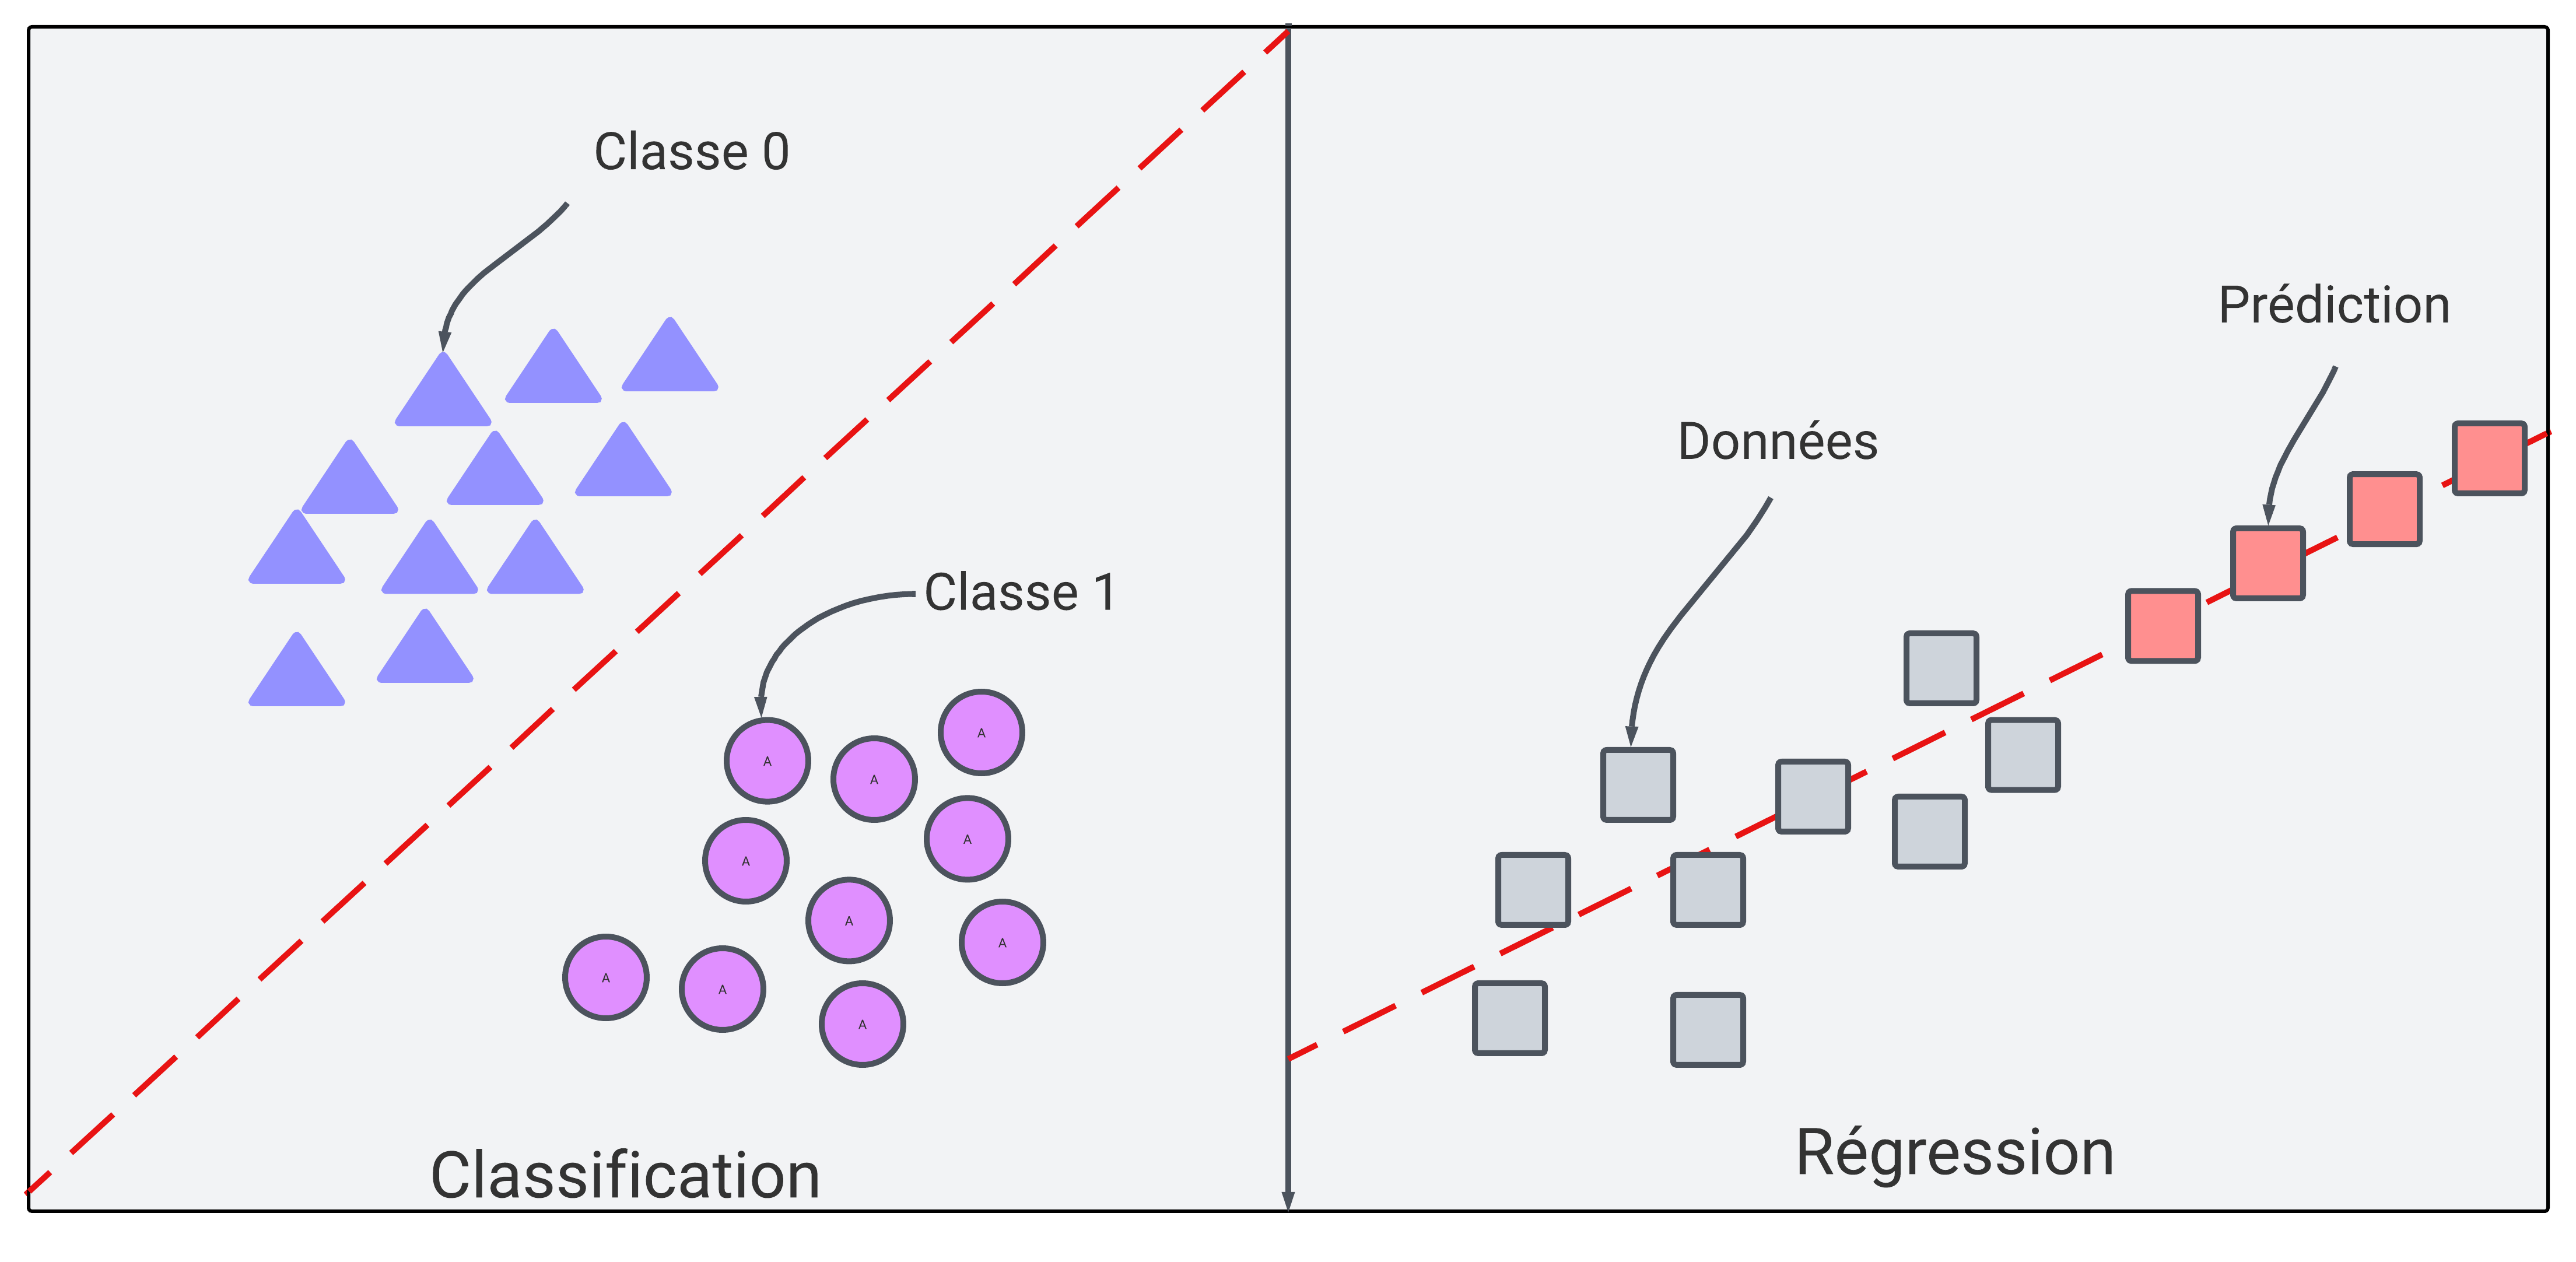
\includegraphics[width=\textwidth]{Figure 2.1.png}
  \caption{Modèles de classification et de régression}
  \label{fig:Modèles de classification et de régression}
\end{figure}



Parmi les algorithmes d’apprentissage supervisé, nous citons : 
\begin{itemize}
   \item[$\bullet$]KNN, SVM, Naïve Bayes, Arbre de décision pour la classification.
    \item[$\bullet$]Régression linéaire ou logistique pour la régression.
   \item[$\bullet$]Les réseaux de neurones pour les deux.
\end{itemize}

\subsection{Apprentissage non-supervisé}
L'apprentissage non-supervisé est une méthode de machine learning où il n'y a pas d'informations préalables sur l'appartenance ou le nombre de classes dans les données d'entraînement. Contrairement à l'apprentissage supervisé, il n'y a pas de labels associés à chaque exemple de données, ce qui signifie que l'algorithme doit trouver des modèles de similitude ou de différence entre les données pour les regrouper en clusters ou les transformer en représentations plus simples et compréhensibles.

Un exemple courant de cette approche est le clustering, qui consiste à regrouper les échantillons similaires en classes ou en groupes (Figure 2.2).
\newpage
\begin{figure}[!h]
  \centering
  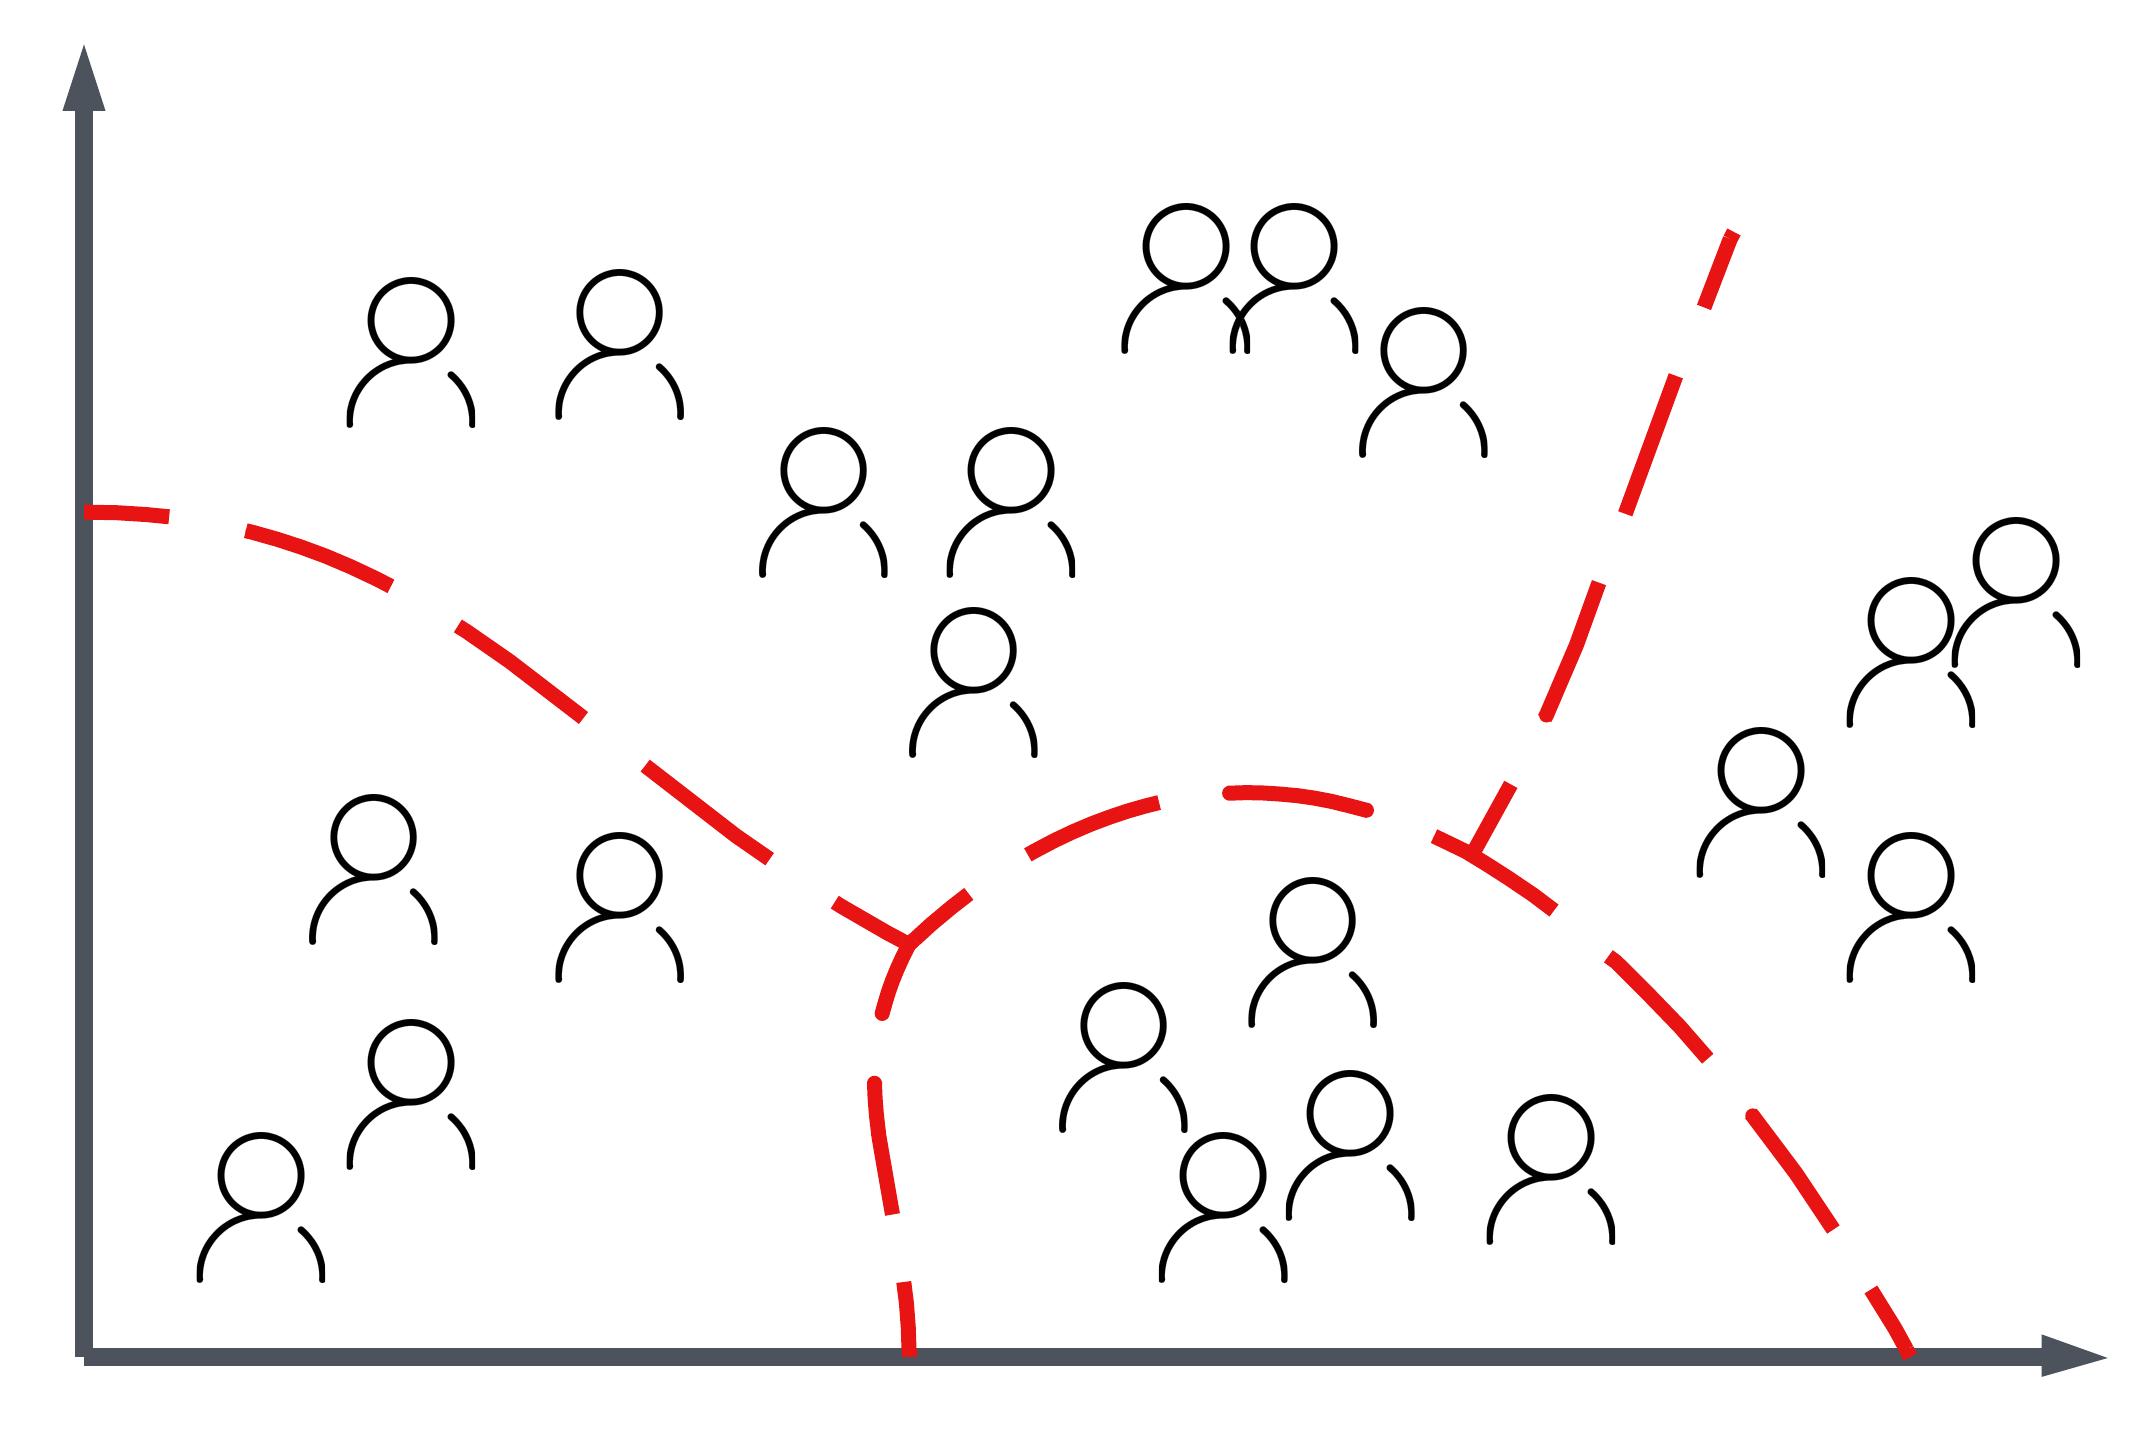
\includegraphics[width=9cm,height=6cm]{Figure 2.2.png}
  \caption{Clustering}
  \label{fig:Clustering}
\end{figure}

Il est également important de souligner que la réduction de dimensions est une étape cruciale pour simplifier les modèles des algorithmes d'apprentissage automatique. L'analyse en composantes principales (ACP) est un exemple d'une technique de réduction de dimensions permettant de passer d'un espace de haute dimension à un espace de dimension réduite, généralement deux ou trois dimensions. Cela permet de visualiser les données de manière plus simple et d'identifier des tendances ou des relations entre les variables qui seraient autrement difficiles à percevoir dans un espace de grande dimension.

Dans la figure 2.3, les attributs des chiffre manuscrits de la base MNIST sont projetées sur 2 axes principaux suite à l'utilisation de l'ACP.
\begin{figure}[!h]
  \centering
  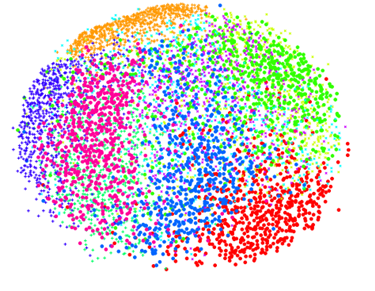
\includegraphics[width=8cm,height=6cm]{Figure 2.3.png}
  \caption{Visualisations des 6000 chiffres manuscrits de la BD MNIST}
  \label{fig:Visualisations des 6000 chiffres manuscrits de la BD MNIST}
\end{figure}
\newpage
\subsection{Apprentissage semi-supervisé}
L'apprentissage semi-supervisé consiste à travailler avec des bases de données où seule une partie des données est étiquetée. Les algorithmes utilisent la similarité entre les données étiquetées et non étiquetées pour regrouper les échantillons dans des classes similaires. Cette approche est intéressante car elle permet de tirer parti de la puissance de l'apprentissage supervisé tout en évitant les coûts élevés liés à l'étiquetage manuel de grandes quantités de données. (Figure 2.4)
\begin{figure}[!h]
  \centering
  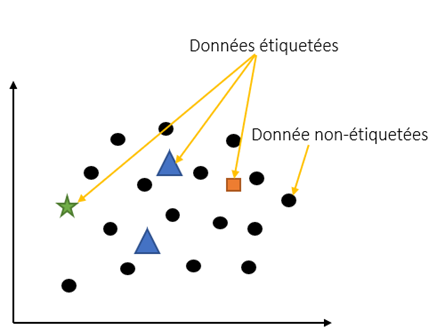
\includegraphics[width=10cm,height=8cm]{Figure 2.4.png}
  \caption{Exemple des données d’entrée pour un algorithme semi-supervisée}
  \label{fig:Exemple des données d’entrée pour un algorithme semi-supervisée}
\end{figure}

\subsection{Apprentissage par renforcement}
L’apprentissage par renforcement est une branche de l'apprentissage automatique qui se concentre sur la prise de décision séquentielle. Dans cette approche, un algorithme apprend à partir de l'interaction avec son environnement en effectuant des actions et en recevant des récompenses ou des pénalités en fonction de la qualité de ses décisions. L'objectif est d'apprendre à prendre les meilleures décisions possibles dans un environnement dynamique et incertain, en maximisant une récompense à long terme.
\clearpage
\section{Apprentissage profond(Deep Learning)}
Le Deep Learning utilise des réseaux de neurones artificiels très profonds pour effectuer des tâches de classification, de prédiction et de génération de données. Les réseaux de neurones profonds sont des réseaux qui ont de nombreuses couches cachées, ce qui leur permet de capturer des relations complexes et non linéaires entre les données d'entrée et de sortie. \\

\begin{itemize}
   \item[$\bullet$]\textbf{Couche d’entrée} : Cette Couche contient les entrées : Texte, valeurs numériques, images...
    \item[$\bullet$]\textbf{Couche cachée} :  Cette couche trouve une relation entre la couche d’entrée et celle de sortie. Le choix de nombre de couches cachées est fait selon a complexité du problème.
     \vspace{0.5em}
   \item[$\bullet$]\textbf{Couche de sortie} : Cette couche est la dernière couche de neurones qui génère les sorties de données.
\end{itemize}

\begin{figure}[!h]
  \centering
  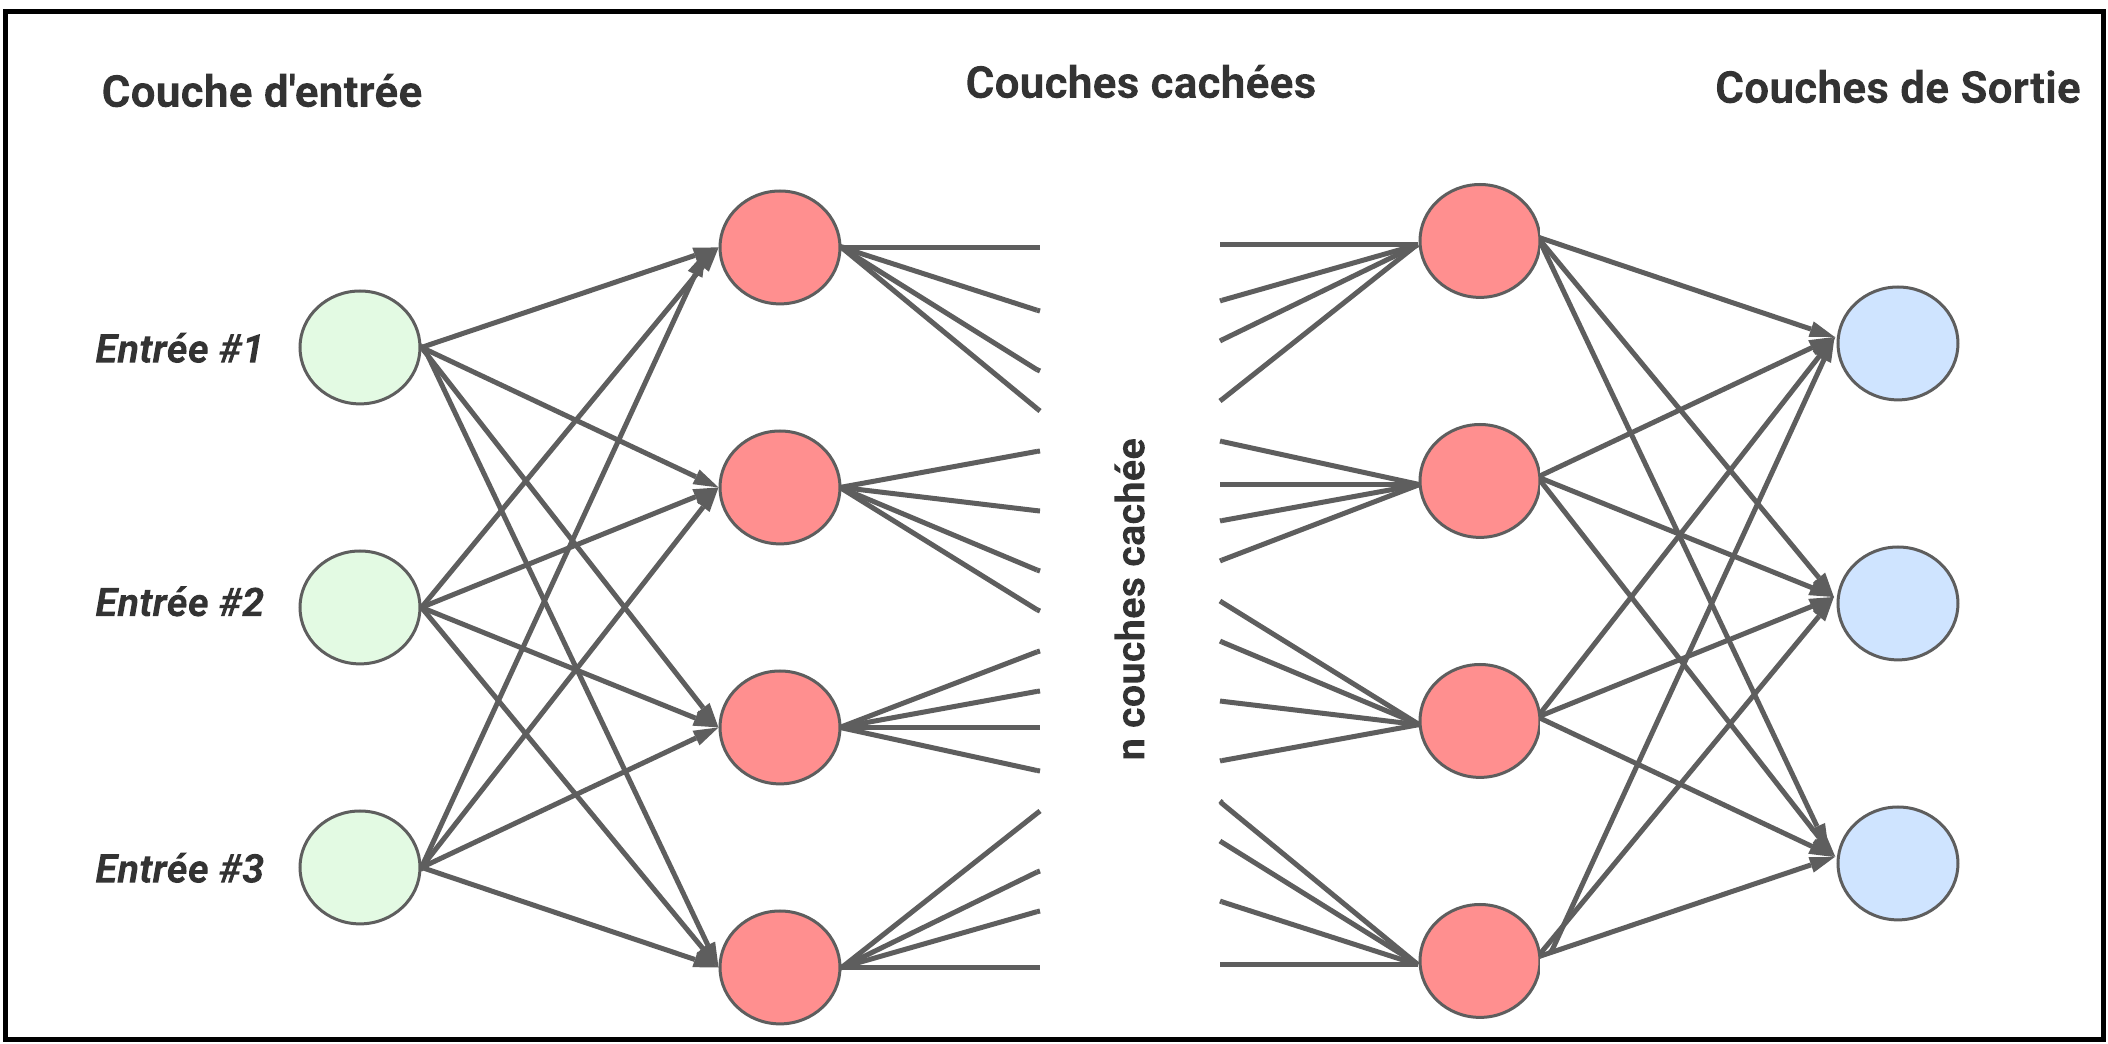
\includegraphics[width=\textwidth]{Figure 2.5.png}
  \caption{Principe du Deep Learning  }
  \label{fig:Principe du Deep Learning  }
\end{figure}

Figure 2.6 présente comment l’apprentissage profond a tendance à bien fonctionner avec de grandes quantités de données, tandis que les modèles d’apprentissage automatique plus traditionnels cessent de s’améliorer à un moment donné.
\clearpage
La performance des réseaux de neurones s'est largement améliorée lorsque les capacités de calcul ont augmenté. Cela a permis d'augmenter le nombre de couches cachées (d'où le nom de deep learning) pour des calculs en un temps acceptable.(Figure 26 \footnote{\shortcite{alom2019state}})
\begin{figure}[!h]
  \centering
  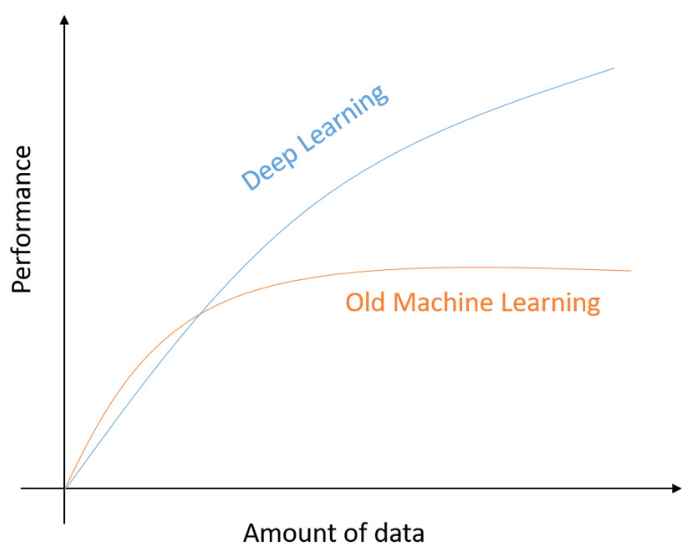
\includegraphics[width=12cm,height=10cm]{Figure 2.6.png}
  \caption{Performance du Deep Learning vs les modèles traditionnels selon la quantité des données.}
  \label{fig:Deep Learning vs les modèles traditionnels. }
\end{figure}
\newline
L'apprentissage profond englobe plusieurs types d'algorithmes, et l'un des plus utilisés est le réseau de neurones convolutifs (CNN en anglais).

\subsection{CNN}
En apprentissage profond, un CNN est une classe de réseaux neuronaux profonds, le plus souvent utilisée pour analyser des images visuelles.
 Lorsque nous pensons à un réseau neuronal, nous pensons à des multiplications de matrices, mais ce n'est pas le cas avec ConvNet. Il utilise une technique spéciale appelée convolution.\\En mathématiques, la convolution est une opération mathématique sur deux fonctions qui produit une troisième fonction qui exprime comment la forme de l'une est modifiée par l'autre.
 \begin{figure}[!h]
  \centering
  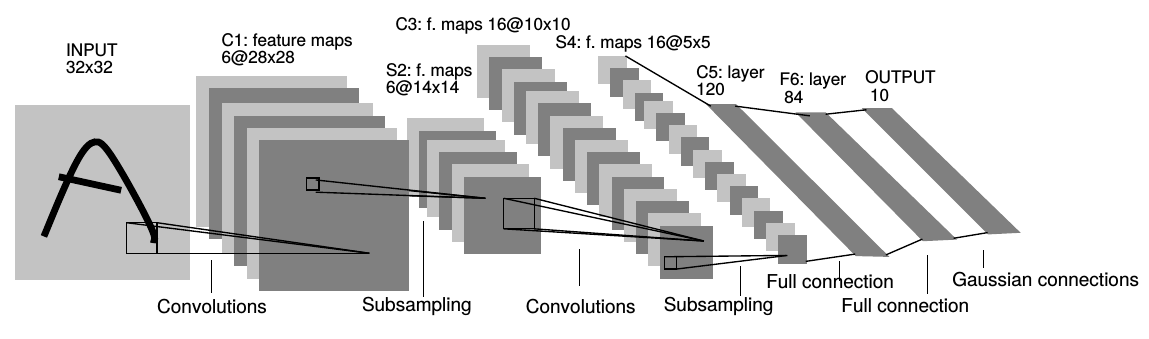
\includegraphics[width=\textwidth]{Figure 2.7.png}
  \caption{Gradient-Based appliqué à la reconnaissance de documents}
  \label{fig:Gradient-Based appliqué à la reconnaissance de docuemnts. }
\end{figure}

La figure 2.7 \footnote{\shortcite{lecun1998gradient}} montre l'architecture d'un réseau de neurones convolutif (ConvNet/CNN) utilisé pour la reconnaissance de caractères manuscrits.
La figure montre une succession de couches de traitement d'informations qui sont organisées de manière hiérarchique, permettant au modèle de capturer des caractéristiques de plus en plus abstraites de l'image en entrée.
\subsubsection{Couches}
Les CNN sont composés de différentes couches qui permettent d'extraire des informations de plus en plus complexes des images en entrée. Plus le nombre de couches est important, plus le modèle est complexe et capable de détecter des caractéristiques plus précises dans l'image.

\begin{itemize}
    \item [$\bullet$]\textbf{Couche de convolution (CONV)}:\\
    La première couche d'un CNN est généralement une couche de convolution, qui permet d'extraire les caractéristiques de l'image en appliquant des filtres sur les pixels de l'image. Cette opération permet de préserver la relation entre les différentes parties de l'image. En utilisant une taille de filtre plus petite que celle de l'image, la taille de l'image est réduite sans perdre la relation entre les pixels. Par exemple, en appliquant une convolution à une image de 5x5 avec un filtre de 3x3 et un pas de 1x1, l'image de sortie sera de 3x3 (soit une réduction de \%64 
    de la complexité de l'image).
    
\par Ces couches de convolution sont donc cruciales pour extraire des informations importantes des images en entrée et sont souvent suivies de couches de sous-échantillonnage (pooling) pour réduire la dimension de la sortie. L'empilement de ces couches permet de construire des modèles de plus en plus complexes et performants pour des tâches de reconnaissance d'images, de détection d'objets, et bien d'autres. (Figure 2.8 et 2.9 \footnote{\shortcite{mnist-image-classification}})
\clearpage
\begin{figure}[!h]
  \centering
  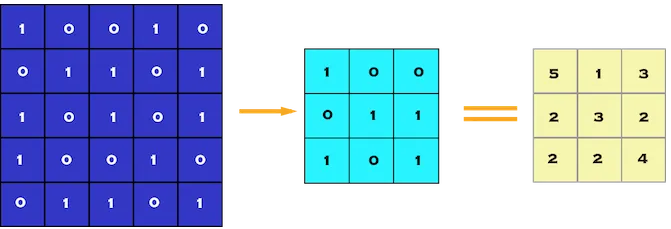
\includegraphics[width=\textwidth]{Figure 2.8.png}
  \caption{Convolution d'une image de 5 x 5 pixels avec un filtre de 3 x 3 pixels (pas de 1 x 1 pixel) }
  \label{fig:CONV}
\end{figure}


 \vspace{0.5em}
    \item [$\bullet$]\textbf{Couche de Pooling  (POOL)}:\\
  La couche de Pooling est une opération généralement appliquée entre deux couches de convolution. Celle-ci reçoit en entrée les features maps formées en sortie de la couche de convolution et son rôle est de réduire la taille des images, tout en préservant leurs caractéristiques les plus essentielles. Parmi les plus utilisés, on retrouve le max-pooling mentionné précédemment ou encore l’average pooling dont l’opération consiste à conserver à chaque pas, la valeur moyenne de la fenêtre de filtre. 
Finalement, on obtient en sortie de cette couche de Pooling, le même nombre de feature maps qu’en entrée mais considérablement compressées
\begin{figure}[!h]
  \centering
  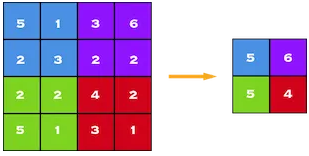
\includegraphics[width=10cm,height=5cm]{Figure 2.9 .png}
  \caption{Max pooling par un facteur de 2 x 2 }
  \label{fig:POOL}
\end{figure}

\newpage
    \item [$\bullet$]\textbf{Couche d’activation ReLU }:\\
  Cette couche remplace toutes les valeurs négatives reçues en entrées par des zéros. L’intérêt de ces couches d’activation est de rendre le modèle non linéaire et de ce fait plus complexe.\\
ReLU désigne la fonction réelle non-linéaire définie par 
$ReLU = max(0,x)$
\begin{figure}[!h]
  \centering
  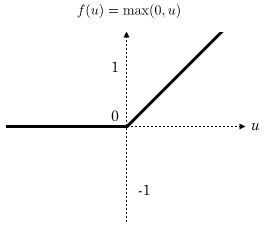
\includegraphics[width=10cm,height=8cm]{Figure 2.10.png}
  \caption{Allure de la fonction ReLU }
  \label{fig:Allure de la fonction ReLU}
\end{figure}

\vspace{0.5em}
    \item [$\bullet$]\textbf{Couche Fully Connected (FC)}:\\
Ces couches sont placées en fin d’architecture de CNN et sont entièrement connectées à tous les neurones de sorties (d’où le terme fully-connected). Après avoir reçu un vecteur en entrée, la couche FC applique successivement une combinaison linéaire puis une fonction d’activation dans le but final de classifier l’input image (voir figure 2.5). Elle renvoie enfin en sortie un vecteur de taille d correspondant au nombre de classes dans lequel chaque composante représente la probabilité pour l’input image d’appartenir à une classe.

\vspace{0.5em}
    \item [$\bullet$]\textbf{Couche de normalisation de lot}:\\
Cette couche normalise les activations des couches précédentes pour accélérer l'apprentissage et améliorer la généralisation.
\vspace{0.5em}
    \item [$\bullet$]\textbf{Couche de dropout }:\\
Cette couche désactive de manière aléatoire certains neurones pendant l'entraînement pour éviter le sur-apprentissage et améliorer la généralisation.
\end{itemize}
\vspace{0.5cm}
Ces couches peuvent être combinées de différentes manières pour construire des architectures de CNN complexes qui sont capables de résoudre une grande variété de tâches de vision par ordinateur.

\subsubsection{Optimiseurs}
Les optimiseurs sont des algorithmes utilisés pour ajuster les poids de chaque couche du réseau de neurones convolutif pendant l'entraînement afin de minimiser la fonction de perte.
La fonction de perte mesure la différence entre les valeurs prédites par le modèle et les vraies valeurs. L'objectif est de minimiser cette différence pour que les prédictions soient aussi précises que possible. Les optimiseurs tels que l'algorithme de descente de gradient stochastique (SGD) ou l'algorithme d'Adam ajustent les poids des couches du réseau de neurones convolutif pour minimiser la fonction de perte.

\section{Paramètres et hyperparamètres du ML et du DL}
Dans ML/DL, les modèles sont définis ou représentés par des paramètres de modèle. Cependant, le processus d’entrainement d'un modèle implique de choisir les meilleurs hyperparamètres. Ceci est utilisé par les algorithmes d'apprentissage pour apprendre les meilleurs paramètres qui mappent correctement les caractéristiques d'entrée aux étiquettes ou aux cibles pour obtenir une certaine forme d'intelligence.
\subsection{Paramètres}
Les paramètres sont internes au modèle. Autrement dit, ils sont appris ou déduits uniquement à partir des données pendant l’entrainement, car l'algorithme utilisé tente d'apprendre les associations entre les caractéristiques d'entrée et les étiquettes ou les cibles. L’entrainement du modèle commence généralement par l'initialisation des paramètres à une certaine valeur (aléatoire ou définie sur zéro). \\Au fur et à mesure de l'apprentissage, les valeurs initiales sont mises à jour à l'aide d'un algorithme d'optimisation (comme gradient descent). Un algorithme d'apprentissage met à jour en permanence les valeurs des paramètres au fur et à mesure qu'il s'entraîne, mais ne modifie pas les valeurs des hyperparamètres définies par le concepteur du modèle. 

A la fin du processus d'apprentissage, les paramètres du modèle constituent le modèle lui-même.
Voici quelques exemples courants :
\begin{itemize}
    \item Les coefficients (ou weights) des modèles de régression linéaire et logistique.
    \item Cluster centroïdes en clustering.
\end{itemize}

Les paramètres de ML/DL sont des valeurs qui peuvent être modifiées et ils sont influencées par le choix des hyperparamètres à fournir. Ainsi, si vous définissez les hyperparamètres avant le début de l'entraînement, l'algorithme d'apprentissage les utilisera pour apprendre les paramètres. 

\subsection{Hyperparamètres}
Dans le ML/DL, un hyperparamètre est tout ce dont la valeur ou la configuration est choisie avant le début de l’entraînement et dont la valeur ou la configuration ne change pas à la fin de la formation. 

Voici quelques exemples courants :
\begin{itemize}
    \item Train-test split ratio.
    \item Nombre de couches cachées.
    \item Nombré d'époques.
    \item Taille du lot.
\end{itemize}

\subsubsection{Taille du lot(Batch size)}
Batch Size est un hyperparamètre qui définit le nombre d'échantillons à traiter avant de mettre à jour les paramètres du modèle interne. Utilisons l'approche la plus simple et comparons les performances des modèles où seule Batch Size varie. (Figure 2.11 \footnote{\shortcite{batchsize_medium}})

\begin{itemize}
    \item Courbe orangée: Batch Size: 64
    \item Courbe bleue: Batch Size: 256
    \item Courbe violette: Batch Size: 1024
\end{itemize}
L'axe des abscisses montre le nombre d'époques d'entraînement, et l'axe des ordonnées est étiqueté pour chaque graphique. Nous observons une tendance claire entre la taille de lot et la précision asymptotique de l'ensemble de test (et d'entraînement). Nous en tirons une conclusion :$\rightarrow$ La taille du lot \textbf{augmente}, la précision du test \textbf{diminue}. 
\clearpage
\begin{figure}[!h]
  \centering
  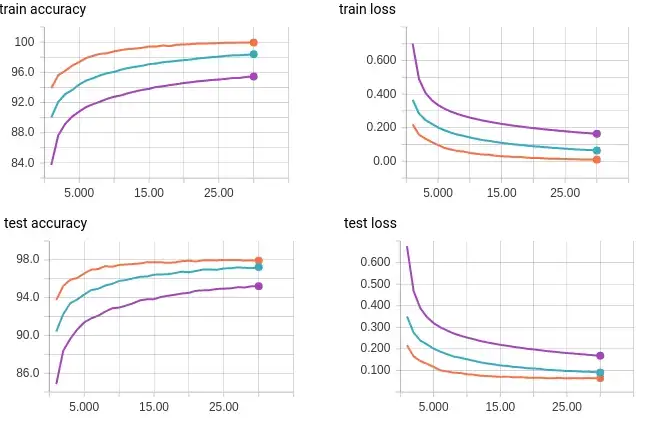
\includegraphics[width=12 cm,height=10cm]{Figure 2.11.png}
  \caption{Précision et perte lors de la variation du Batch Size  }
  \label{fig:Batch Size}
\end{figure}


\subsubsection{Époques}
Dans l'apprentissage automatique, une époque est une passe complète d'un ensemble de données d'entraînement à travers un réseau de neurones. En d'autres termes, l'algorithme d'apprentissage examine tous les exemples d'entraînement une fois. Les époques sont donc une mesure de l'itération de l'ensemble des données d'entraînement. En règle générale, plus le nombre d’époques est élevé, plus le modèle est entraîné. Cependant, il est important de noter que l'augmentation du nombre d’époques n'entraîne pas toujours une amélioration des performances du modèle. En effet, l'overfitting peut se produire si le modèle est trop entraîné sur les données d'entraînement. (Figure 2.12\footnote{\shortcite{deepai_epoch}}). Par conséquent, il est important de déterminer le nombre optimal d’époques pour entraîner le modèle. Cela peut être fait en utilisant des techniques d'optimisation d'hyperparamètres telles que la recherche par grille, la recherche aléatoire ou la recherche bayé-sienne.
\clearpage
\begin{figure}[!h]
  \centering
  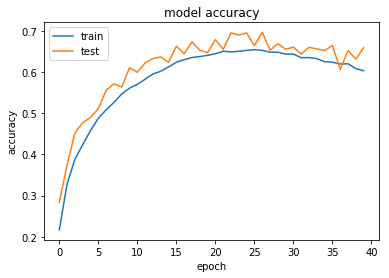
\includegraphics[width=12 cm,height=8cm]{Figure 2.12.png}
  \caption{La précision d’un modèle en fonction de nombre d’époques}
  \label{fig:Epoque}
\end{figure}

\vspace{1cm}

\begin{itemize}
    \item [$\bullet$]\textbf{La recherche par grille}:\\
    Cette méthode a été introduite dans le domaine de l'optimisation des hyperparamètres dans les années 1960 par un statisticien américain du nom de Marvin Zelen.\\
Elle consisterait à tester différents nombres d'époques pour entraîner le modèle. Les performances du modèle seraient évaluées pour chaque combinaison d'hyperparamètres en utilisant une métrique d'évaluation telle que la précision (accuracy) ou la perte (loss).\\
Cependant, la recherche par grille peut être coûteuse en termes de temps et de ressources, surtout lorsque le nombre d'hyperparamètres et de valeurs à tester est élevé. 

\vspace{1cm}
\item [$\bullet$]\textbf{La recherche bayésienne }:\\
Cette méthode est une méthode d'optimisation des hyperparamètres qui permet de trouver les valeurs optimales pour les hyperparamètres d'un modèle en utilisant une approche probabiliste. Cette méthode a été introduite dans un article de 1997 intitulé "Bayesian optimization for machine learning" par David J.C. MacKay.\\
Depuis lors, la recherche bayésienne est devenue une méthode populaire pour l'optimisation des hyperparamètres dans le domaine de l'apprentissage automatique. Elle est couramment utilisée pour trouver les valeurs optimales pour des hyperparamètres tels que le taux d'apprentissage, le nombre de couches cachées, la taille du lot, etc.\\
 Cette méthode présente également certains points négatifs. Tout d'abord, elle nécessite un temps de calcul plus important que la recherche par grille car elle doit effectuer plusieurs évaluations de modèle. De plus, elle nécessite de spécifier une distribution de probabilité initiale sur les hyperparamètres, ce qui peut être difficile à faire dans certains cas. Enfin, la méthode est sensible aux choix d'hyperparamètres initiaux et de la fonction d'acquisition utilisée pour sélectionner les prochaines valeurs d'hyperparamètres à évaluer.
\end{itemize}
\vspace{1.25cm}
\section{Conclusion}
En conclusion, le DL, et en particulier CNN, ont apporté des avancées majeures dans le domaine de l'apprentissage automatique pour l'analyse d'images et de vidéos. Les hyperparamètres, tels que le nombre d'époques, jouent un rôle crucial dans la performance de ces modèles.\\
Cependant, l'estimation du nombre optimal d'époques reste un défi important pour les praticiens de l'apprentissage automatique. C'est pourquoi de nouvelles techniques sont nécessaires pour déterminer le nombre d'époques optimal de manière plus précise et plus efficace.\\
Dans ce chapitre, nous avons exploré l'état de l'art des hyperparamètres, en nous concentrant sur les époques, et avons discuté de l'importance de l'optimisation de ces paramètres pour améliorer les performances des modèles.\\
Nous avons également ouvert la porte à de nouvelles approches pour déterminer le nombre optimal d'époques, en utilisant des techniques d'estimation de densité de probabilité non paramétriques pour développer une nouvelle métrique d'évaluation.\\
Cette nouvelle approche pourrait offrir de nouvelles perspectives pour optimiser les modèles CNN et améliorer leurs performances. Il reste cependant du travail à faire pour développer et valider cette approche, mais elle pourrait contribuer à une meilleure compréhension des hyperparamètres et à une amélioration significative de la performance des modèles.
